\begin{figure*}[!htb]
\minipage{0.31\textwidth}
  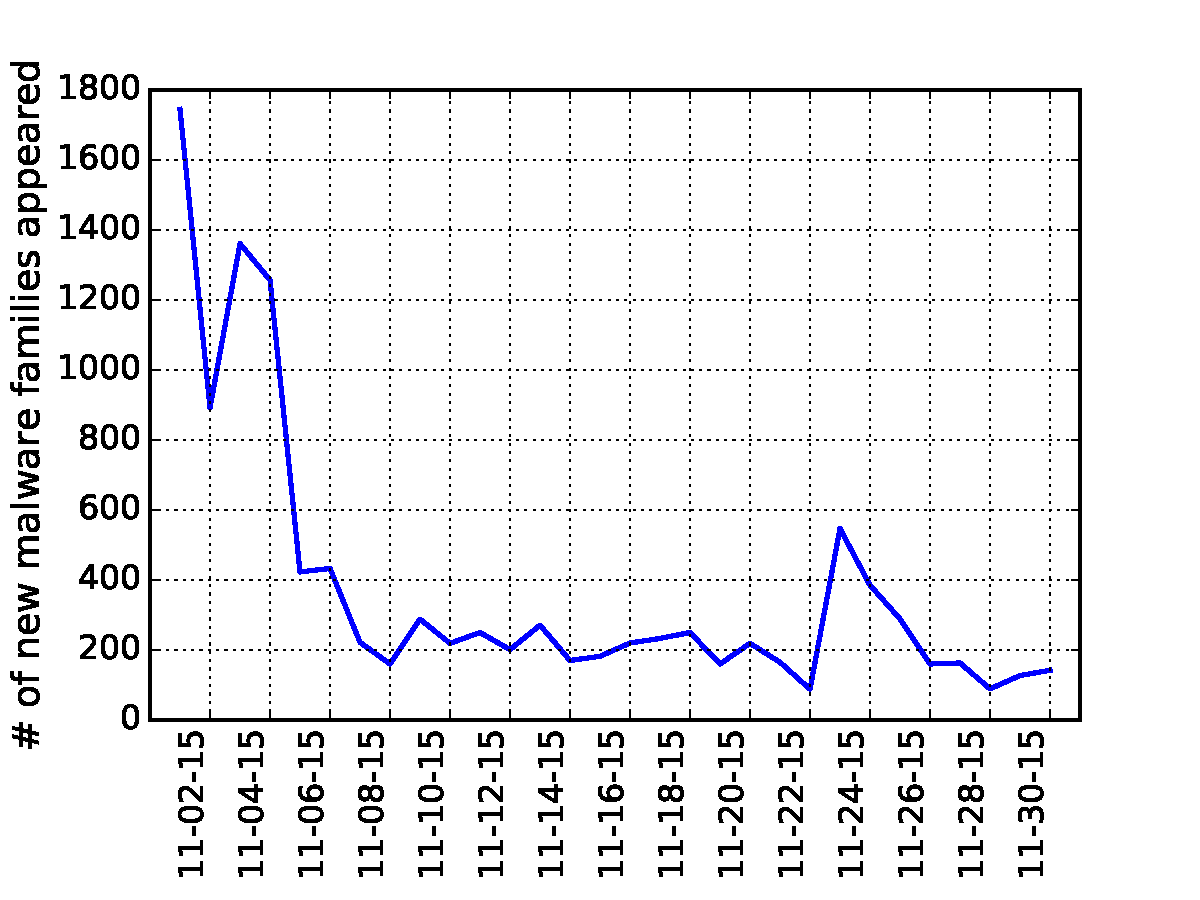
\includegraphics[width=\linewidth]{figure/new_family}
\mycaption{fig:new}{New malware families on VirusTotal in November 2015.}
{
The number of new malware families we observed every day in November 2015.
}
  %\label{fig:overlap}
\endminipage\hfill
\minipage{0.31\textwidth}
  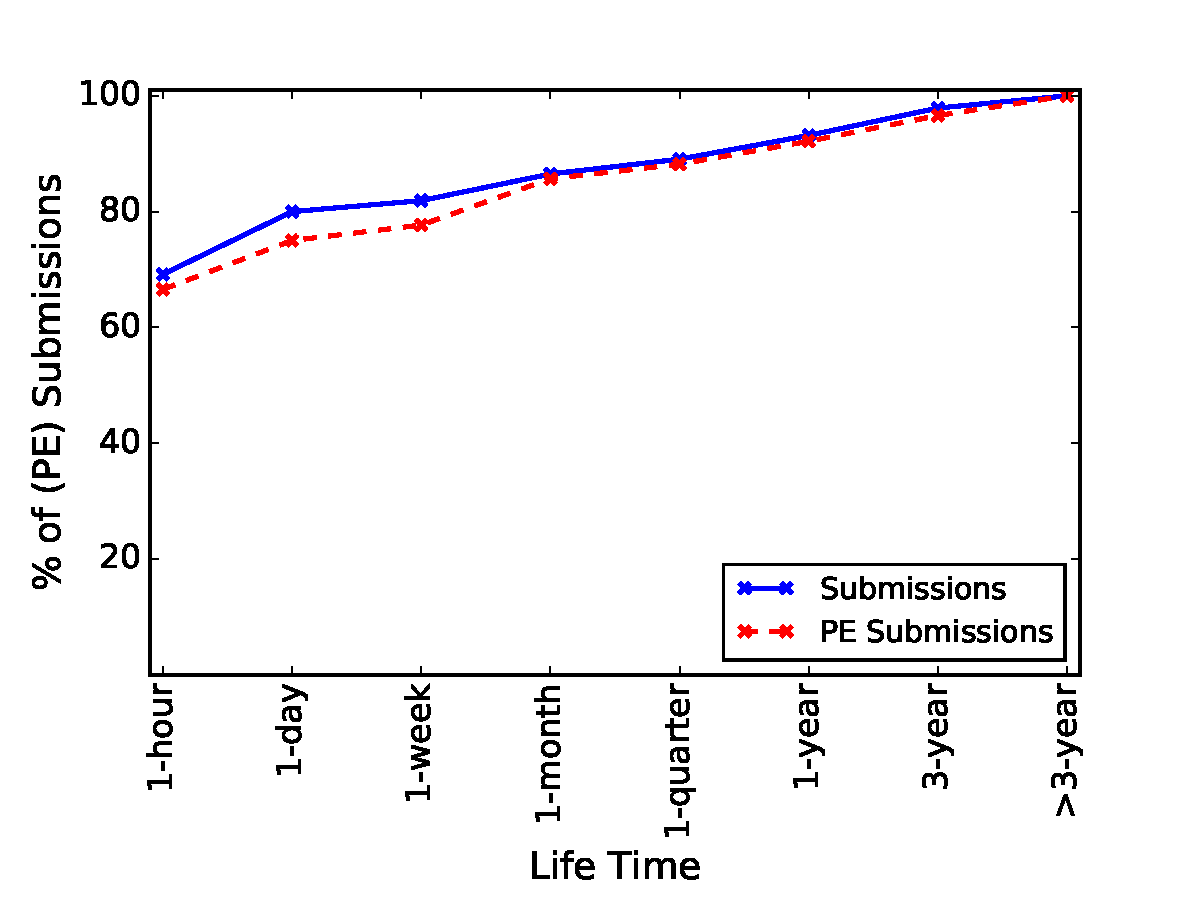
\includegraphics[width=\linewidth]{figure/lifetime}
 \mycaption{fig:life}{Malwares' lifetime in November 2015.}
{
Accumulation distribution of malwares' lifetime in November 2015.
}
  %\label{fig:maxUncover}
\endminipage\hfill
\minipage{0.31\textwidth}%
  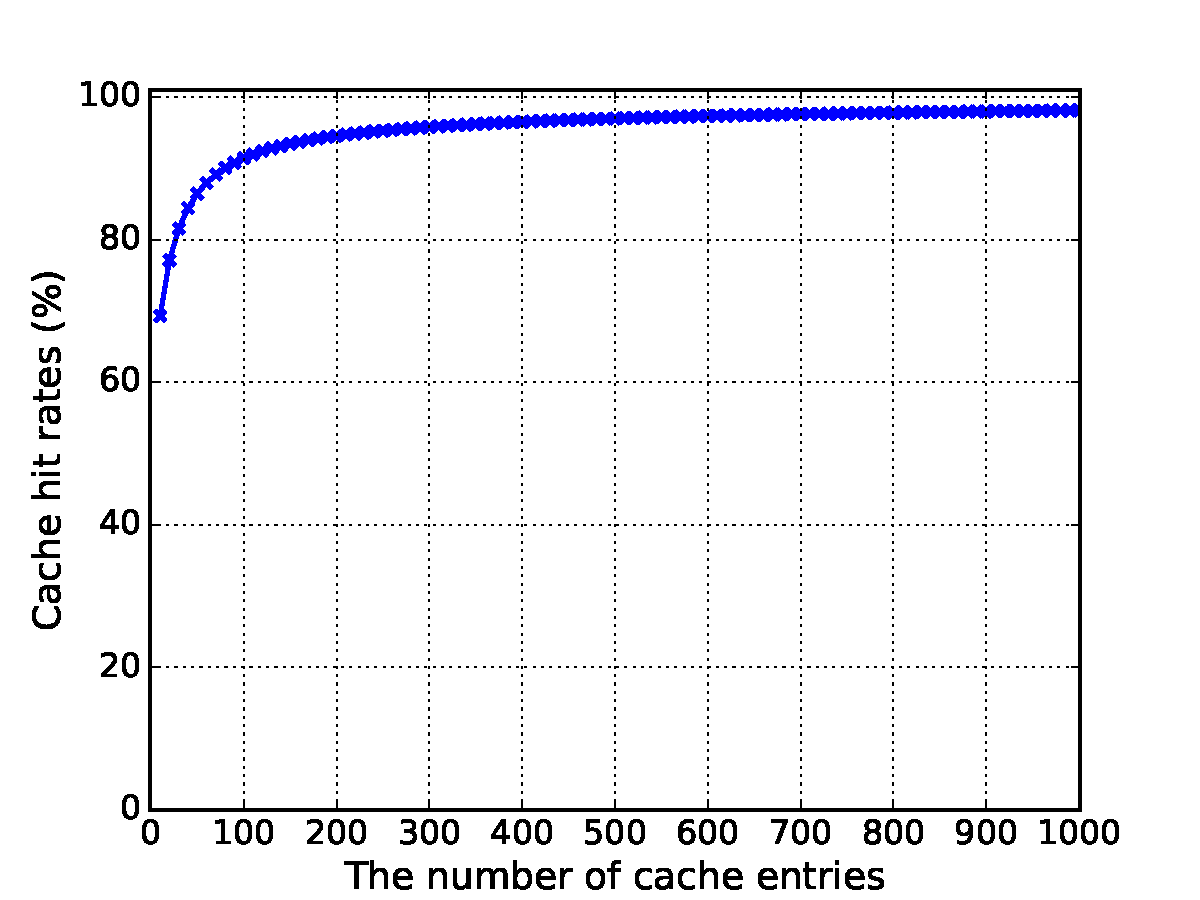
\includegraphics[width=\linewidth]{figure/LRU}
  \mycaption{fig:cache}{Relation between cache hit rate and cache size.}
{Cache hit rate under different values of cache size from 10 to 1000.}
  %\label{fig:aveUncover}
\endminipage\hfill

\vspace{-0.1in}
\end{figure*}

\begin{figure*}[!htb]
\minipage{0.31\textwidth}
  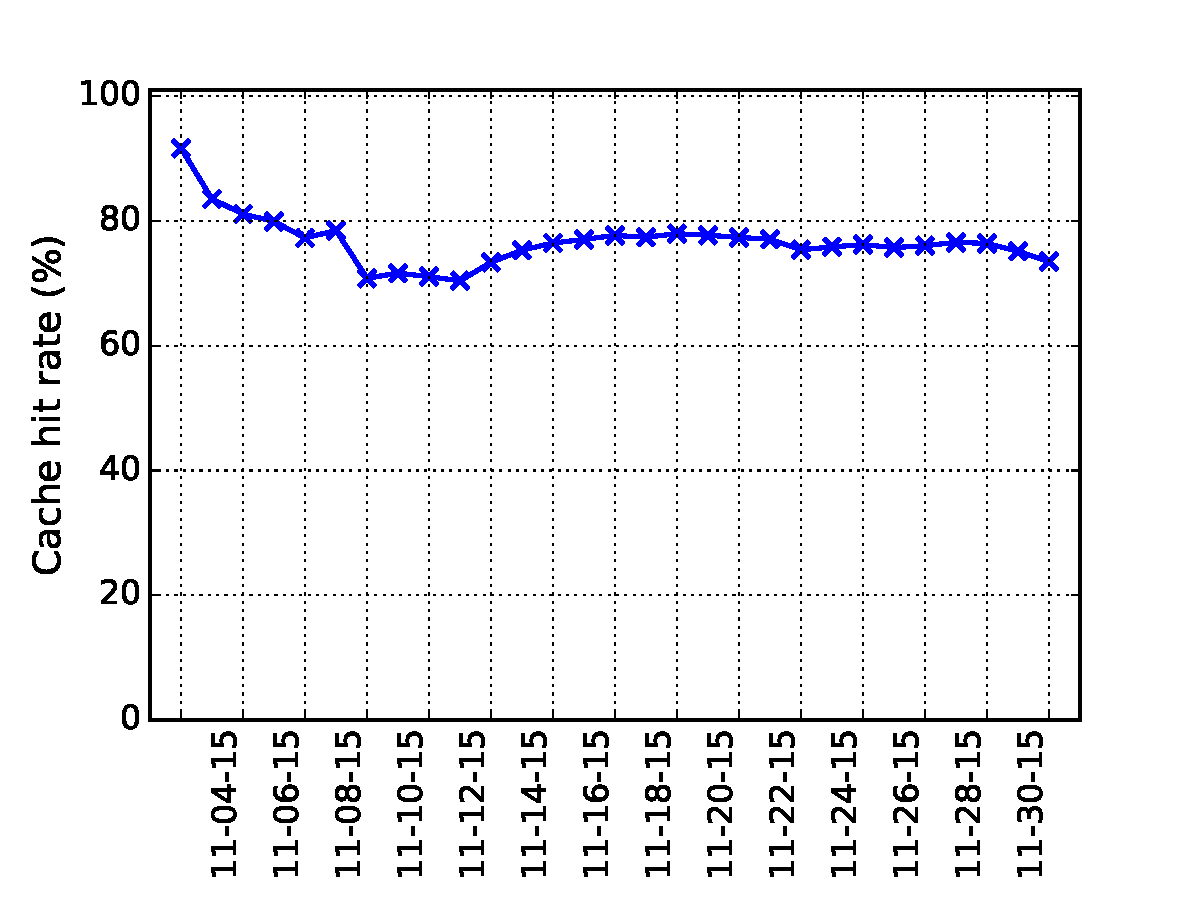
\includegraphics[width=\linewidth]{figure/LRU_day}
\mycaption{fig:batchcache}{Cache hit rate in November 2015.}
{
Cache hit rate every day in November 2015 if we only update cache content at the end of every day.
}
  %\label{fig:overlap}
\endminipage\hfill
\minipage{0.31\textwidth}
  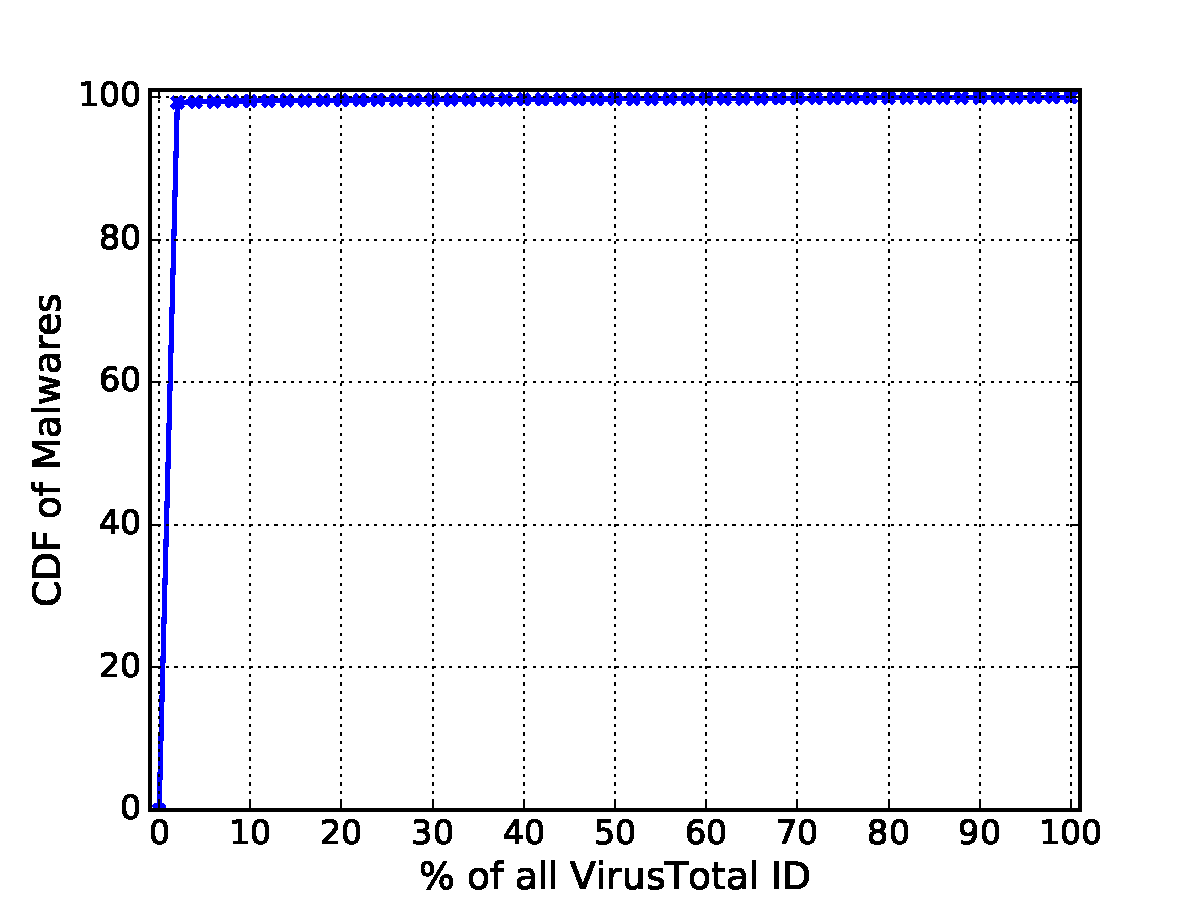
\includegraphics[width=\linewidth]{figure/id}
 \mycaption{fig:id}{Skewness of malware submissions from different users in November 2015.}
{Accumulation distribution of malwares submitted by different users in November 2015.}
  %\label{fig:maxUncover}
\endminipage\hfill
\minipage{0.31\textwidth}%
  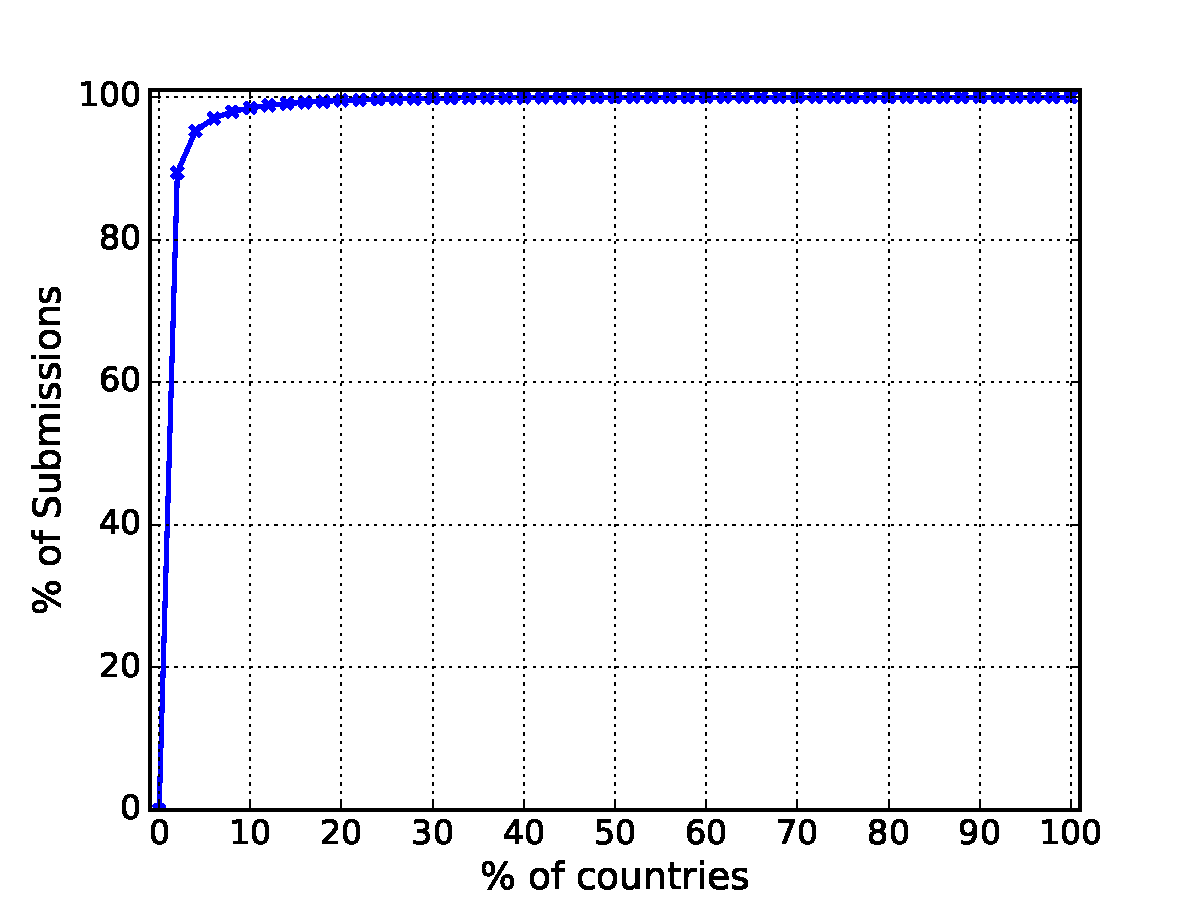
\includegraphics[width=\linewidth]{figure/country}
  \mycaption{fig:country}{Skewness of malware submissions from different countries in November 2015.}
{Accumulation distribution of malwares submitted from different countries in November 2015.}
  %\label{fig:aveUncover}
\endminipage\hfill

\vspace{-0.1in}
\end{figure*}